
\section{Паяльное оборудование}

\subsection{Паяльник}

Паяльник\ --- обязателен дешевый сетевой мощностью не менее 20\,Вт, типа
ЭПСН-25/220. Ограничитель мощности или регулятор температуры легко собрать
самостоятельно.

Для сборки электроники хорошо также иметь маленький монтажный 12\,В 8\,Вт от
паяльной станции ZD-927 ($\sim$100\,р), без самой станции. Если не жалко 500\,р,
берите станцию ZD-927 целиком, внутри простейший регулятор мощности, и вам не
понадобится источник питания на 12\,В, который вы еще не сделали.

\noindent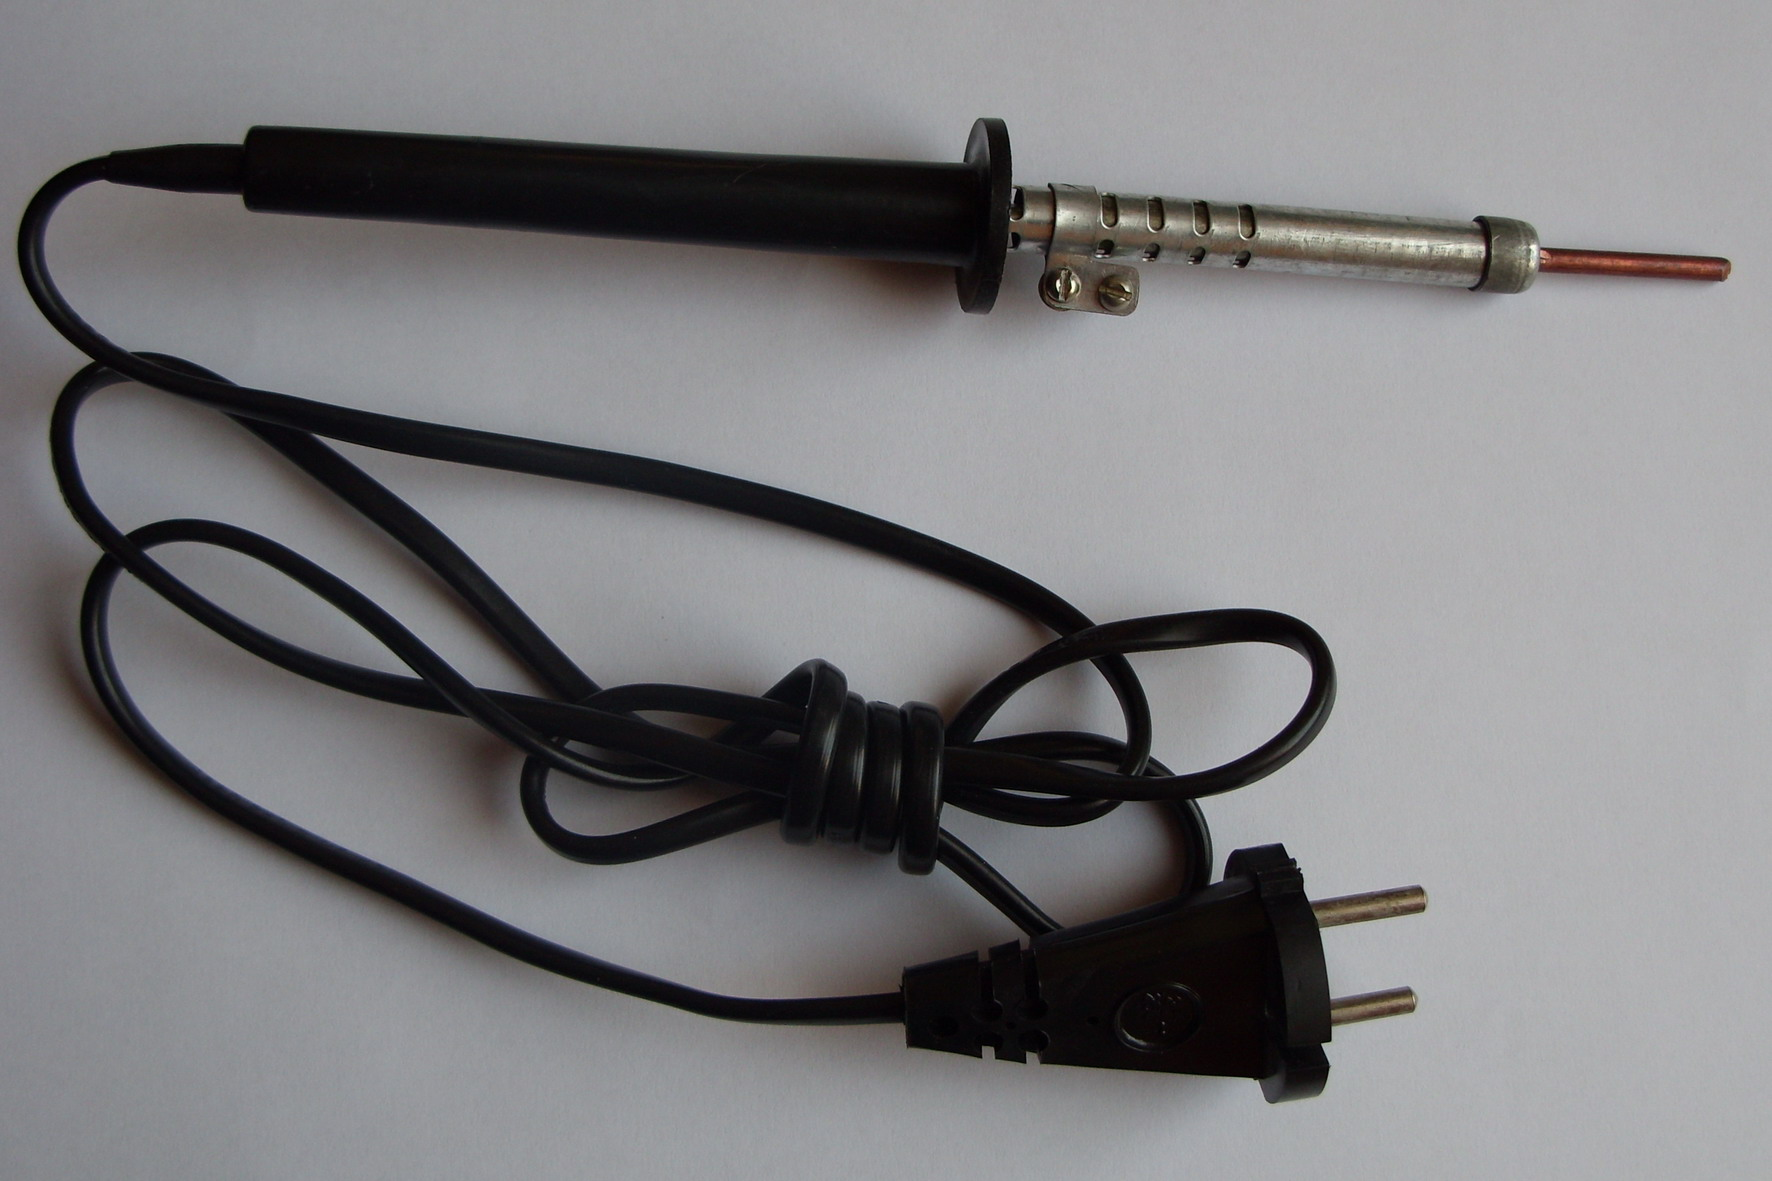
\includegraphics[width=0.4\textwidth]{tech/tools/solder/EPSN25.jpg}
\textbf{Паяльник ЭПСН-25/220}

\noindent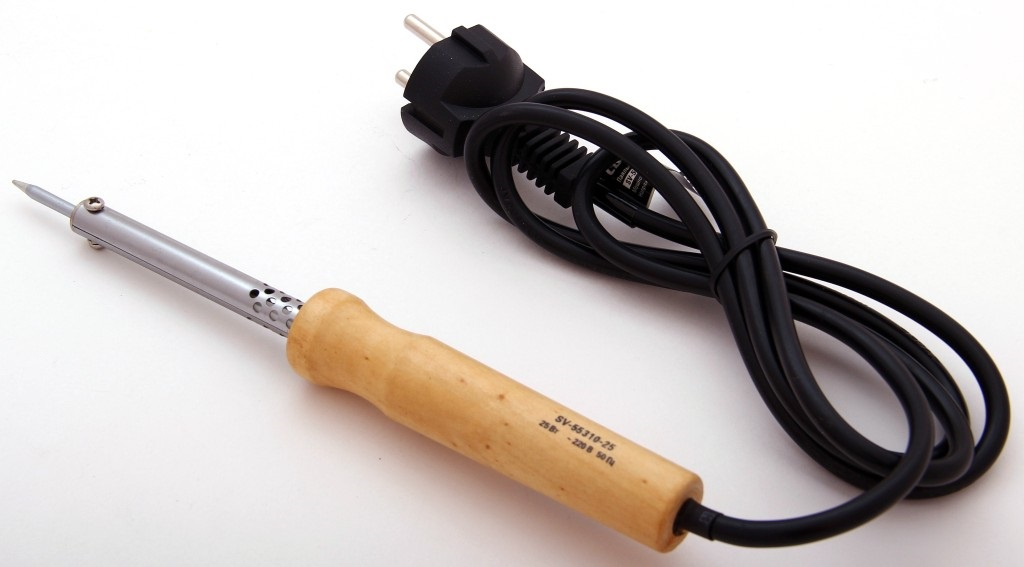
\includegraphics[width=0.4\textwidth]{tech/tools/solder/SV-55310-25.jpg}
\textbf{Паяльник 220В 25Вт, СВЕТОЗАР, SV-55310-25 230\,р.}

\noindent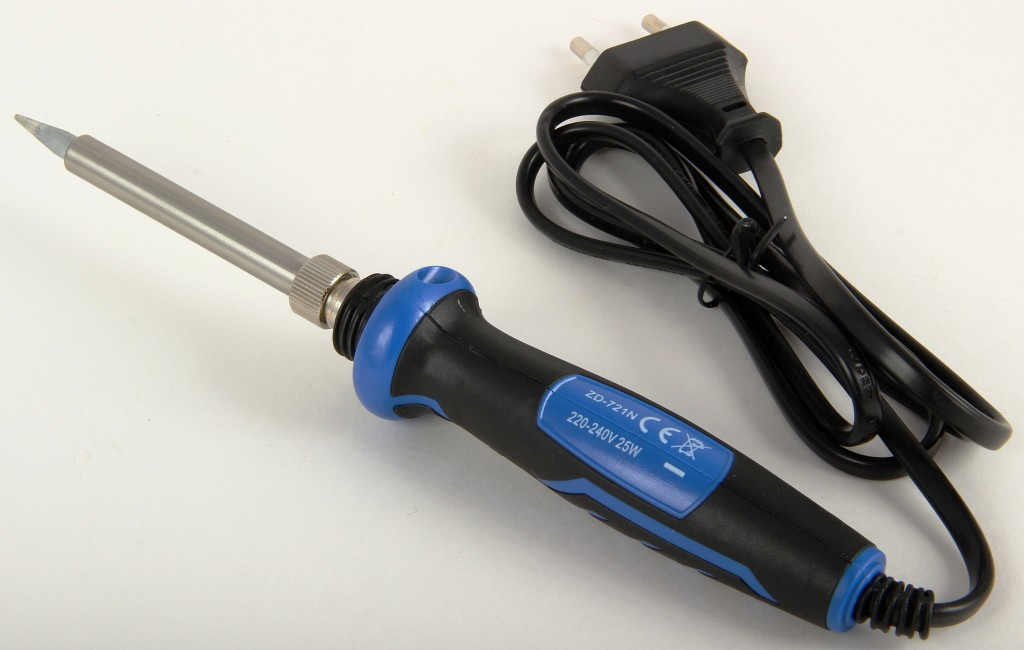
\includegraphics[width=0.4\textwidth]{tech/tools/solder/ZD-721N.jpg}
\textbf{Паяльник 220В 25Вт ZD-721N 175\,р.}

\noindent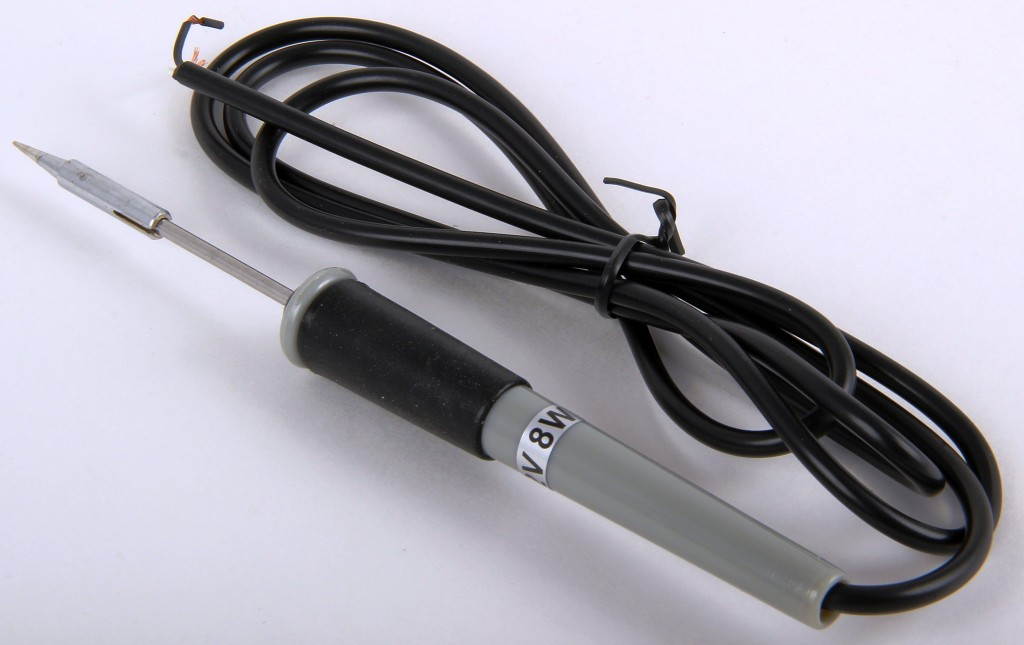
\includegraphics[width=0.4\textwidth]{tech/tools/solder/Iron8W.jpg}
\textbf{Паяльник для станции ZD-927 12\,В 8\,Вт 85\,р.}

\subsection{Паяльная станция}

Из всего разнообразия для хоббита оптимальным являются паяльные станции Lukey
702/853D (3000+\,р). Для работы или регулярного хобби паяльная станция с феном,
а может даже и встроенным источником питания, вещь незаменимая, и не такая уж
дорогая.

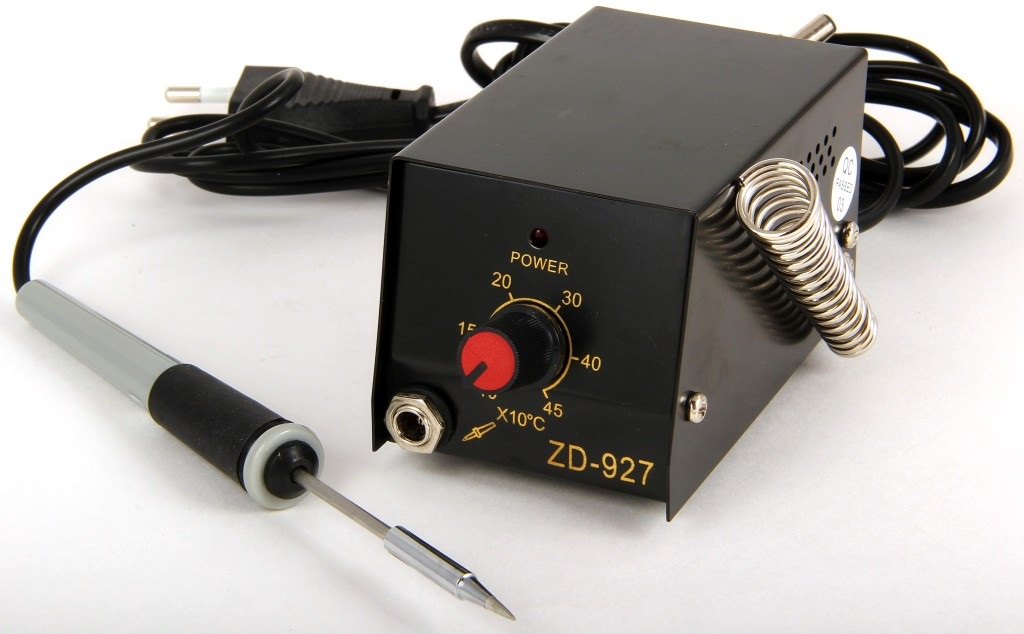
\includegraphics[width=0.45\textwidth]{tech/tools/solder/ZD927.jpg}
\textbf{Паяльная станция ZD-927 520\,р.}

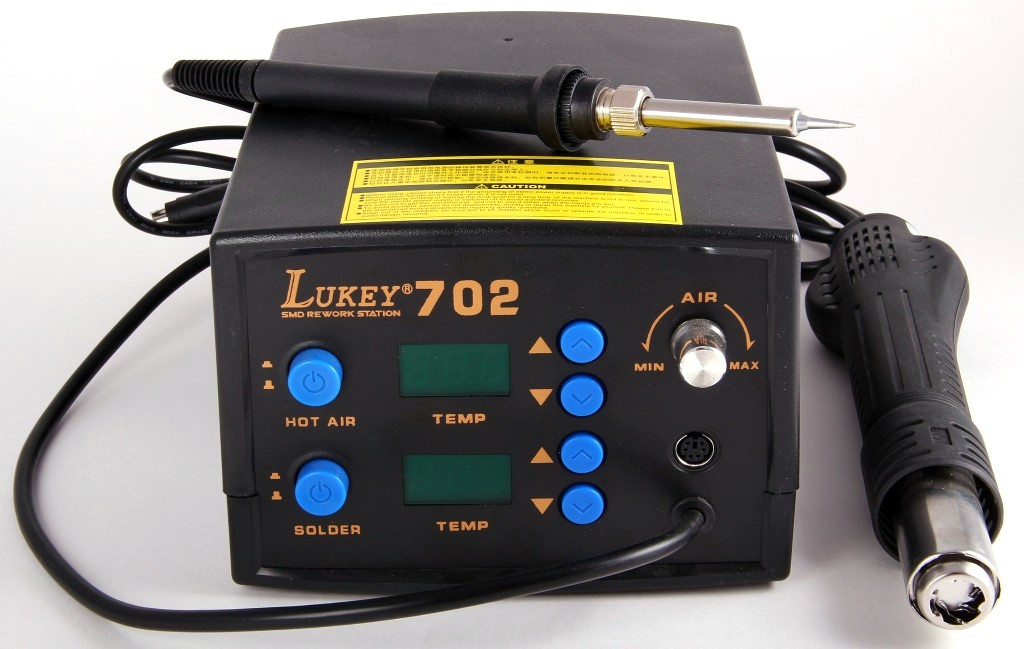
\includegraphics[width=0.45\textwidth]{tech/tools/solder/Lukey702.jpg}
\textbf{Паяльная станция LUKEY 702 3100\,р.}

\clearpage
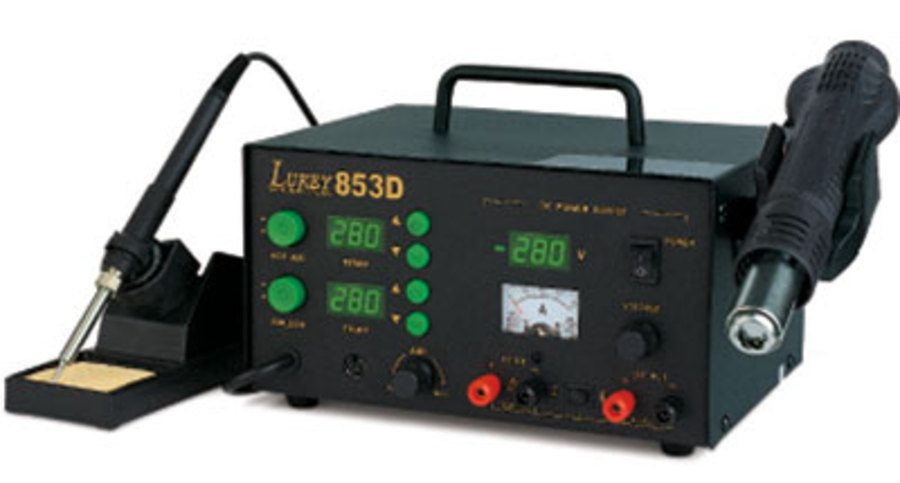
\includegraphics[width=0.95\textwidth]{tech/tools/solder/Lukey853D.jpg}

\textbf{Паяльная станция LUKEY 853D с источником питания 5200\,р.}
\clearpage

